\documentclass{beamer}
\setbeamertemplate{navigation symbols}{} % eliminate navigation bar
\usetheme{CambridgeUS}

\usefonttheme{structurebold}
% Arch Linux Color Theme
\definecolor{arch}{RGB}{23,147,209}
\usecolortheme[named=arch]{structure}
\usecolortheme{whale}
\setbeamercolor{frametitle}{bg=arch!80!black}
\setbeamercolor{title}{bg=arch!90!black}

%% SET BEAMER TEMPLATE
%\setbeamertemplate{headline}

\usepackage{lmodern}
\usepackage{ngerman}
\usepackage[latin1]{inputenc}
\usepackage[naustrian,ngerman]{babel}

\beamersetuncovermixins{\opaqueness<1>{25}}{\opaqueness<2->{15}}


%% META INFORMATION ABOUT DOCUMENT
% \title[short]{long}
% short argument is used in places where there is little space
% long is used on the title slide

\title[Impedanzspektrometer]{Bau eines Impedanzspektrometers mit dem AD5933}
\subtitle{Bachelorarbeit SS2014}
\institute[]{Institut f�r Mikroelektronik und Mikrosensorik \\ Johannes-Kepler-Universit�t Linz}

\subject{AD5933 Impedanzspektrometer}

% ENTER YOUR NAME, SHORT VERSION FOR FOOTER
\author[Feichtinger]{Peter Feichtinger\texorpdfstring{\\}{, } Betreuer: DI Stefan Clara} % Variante: \and

\date{19. M�rz 2014}


\begin{document}

%% TITLE PAGE
\begin{frame}
  \titlepage
\end{frame}

% for longer presentations table of contents is useful
% \begin{frame}
%    \frametitle{Outline} 
%    \tableofcontents          % optional: [pausesections]
% \end{frame}


\section{Thema der Bachelorarbeit}  % always defined outside a frame, optional short argument
\begin{frame}[t]
  \frametitle{Aufgabenstellung}

  \begin{columns}
    \begin{column}{0.6\textwidth}
      \begin{itemize}
        \item Erweiterungsm�glichkeiten des AD5933 analysieren
        \item Entwurf und Realisierung einer Schaltung
        \item Verbindung zum PC mittels STM32F4 Discovery Board und Auswertung in MATLAB
        \item Eventuell eigene Ethernet Schnittstelle
      \end{itemize}
      \vspace{3cm}
    \end{column}
    
    \begin{column}{0.35\textwidth}
      \includegraphics[height=15em]{bilder/stm32.jpg} \\
      \footnotesize{STM32F4 Discovery Board}
    \end{column}
  \end{columns}
\end{frame}

% \pause can be used to uncover elements later
% doesn't work with align

% allowframebreaks, use rarely


\begin{frame}[t]
  \frametitle{AD5933 Impedance Converter Network Analyzer}

  \begin{itemize}
    \item Ansteuerung per $ I^2C $
    \item Liefert Real- und Imagin�rteil der Impedanz
    \item Einfache Aufnahme des Frequenzgangs
  \end{itemize}
  
  \vspace{1em}
  \centering
    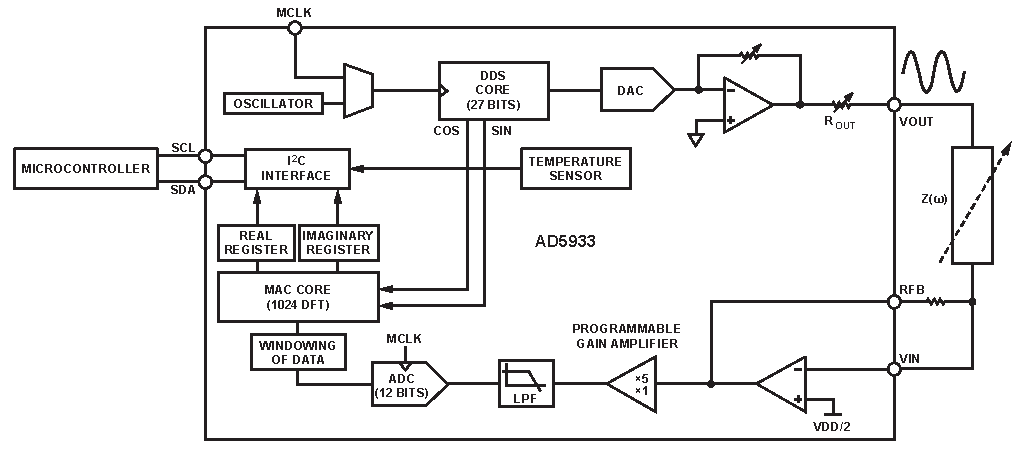
\includegraphics[height=11em]{bilder/ad_block.pdf} \\
  \footnotesize{AD5933 Blockschaltbild}
\end{frame}


\begin{frame}[t]
  \frametitle{M�gliche Erweiterung}
  
  \begin{itemize}
    \item Eigenst�ndige Benutzeroberfl�che mit TI AM335x Starter Kit
    \item Netzwerkanbindung per Ethernet oder WLAN
    \item Export der Daten auf USB-Stick
  \end{itemize}
  
  \vspace{1em}
  \centering
    \includegraphics[height=11em]{bilder/am335x.jpg} \\
  \footnotesize{AM335x Starter Kit}
\end{frame}


%\begin{frame}
  %\centering
  %Vielen Dank f�r Ihre Aufmerksamkeit!
%\end{frame}


\end{document}